%!TEX root = ../../root.tex

\emph{Batch normalization} is a method of \emph{adaptive reparametrization}, motivated by the difficulty of training very deep models. Very deep models involve the composition of several functions or layers. The gradient tells how to update each parameter, under the assumption that the other layers do not change. In practice, we update all of the layers simultaneously.

Consider a layer of a multi-layer perceptron (MLP):
\begin{equation}
    \mathbf{x}^{(k)} = \sigma\left( \mathbf{W}^{(k)} \mathbf{x}^{(k-1)}  \right).
\end{equation}

At each layer the distribution of the input that enters that layer changes all the time during training, since the weights $\mathbf{W}$, and in particular the weights $\vb{W}^{(1:k-1)}$ of the earlier layers change continuously, because it is what we are optimizing over. This phenomenon is called \emph{internal covariate shift}.

It becomes a problem because the layers need to continuously adapt to the new distribution. This leads to slower training of the network than it could be if the input distribution did not change, since in that case the network would not have to account for this change.

Batch normalization is designed to try and \emph{fix} the input distribution at each layer. This is done by \emph{normalizing} the input features at a layer $k$ by the statistics (\emph{mean} and \emph{variance}) computed on the entire training set after it has passed through the network and reached the $k$-th layer.
\begin{equation}
    \hat{\mathbf{x}} = \mathrm{normalize}(\mathbf{x}, \mathcal{X})
\end{equation}
where both $\mathbf{x}$ and $\mathcal{X}$ (all the training set) are parametrized by $\mathbf{W}$ because
both of them have passed through the network until the layer $k$.

So the transformation $normalize(\cdot, \mathcal{X})$ is another transformation that the network must do, therefore to be able to train the network via a gradient descent-like algorithm we will need backprop to be able to propagate gradients through it, i.e. we need the transformation to be \emph{differentiable}, to admit partial derivatives
\begin{equation}
    \frac{\partial}{\partial \mathbf{x}} \mathrm{normalize}(\mathbf{x}, \mathcal{X})\,, \quad\quad \frac{\partial}{\partial \mathcal{X}} \mathrm{normalize}(\mathbf{x}, \mathcal{X})
\end{equation}
needed for the chain rule.

\paragraph{The transformation}

Let's see in detail what $normalize(\cdot, \mathcal{X})$ looks like. 

In the univariable case, normalizing an input variable (also called \emph{standardization} or \emph{whitening}) would mean transforming this variable in order to obtain a mean of $0$ and a variance of $1$. This is done by removing the \emph{mean} over the training set and dividing by the \emph{standard deviation} over the training set:
\begin{equation}
    \mathbf{x} \mapsto \frac{ \mathbf{x} - \mathbb{E}_{\mathbf{x} \in \mathcal{X}}[\mathbf{x}]}{\sqrt{\mathrm{var}_{\mathbf{x} \in \mathcal{X}}[\mathbf{x}]}}.
\end{equation}

% However, we deal with deep models that in general receive inputs described in terms of many features, represented by vectors. 

% The concept of mean remains unchanged, the mean of a vector $\vb{x} \in \mathbb{R}^n$ is just the vector of the mean of all its components.
% \begin{equation}
%     \mathbb{E}_{\vb{x} \in \mathcal{X}}[\vb{x}] = \mqty(\mathbb{E}_{x_1 \in \mathcal{X}_1}[x_1], \dots, \mathbb{E}_{x_n \in \mathcal{X}_n}[x_n])^{\top}
% \end{equation}

% On the other hand, the concept of variance is replaced by \emph{covariance}, since in a multivariate distribution we are not only interested in the \emph{variability} of a single variable (how far from the mean it can go) but also in the \emph{joint variability} of every pair of variables in the distribution. It may be frequent to observe single variables going far from the mean, when the other are kept fixed, but it may be very unfrequent to observe a certain pair of variables to go far from the mean \emph{jointly}, i.e. at the same time. 
% For this reason, we cannot describe (co)variance in the multivariable setting with a simple vector, but we need the \emph{covariance matrix}:
% \begin{equation}
%    \mathrm{cov}[\vb{x}] = \underbrace{\mathbb{E}_{\vb{x} \in \mathcal{X}}[\vb{x} \vb{x}^{\top}]}_{\mathclap{\text{mean of the outer product}}} - \overbrace{\mathbb{E}_{\vb{x} \in \mathcal{X}}[\vb{x}] \mathbb{E}_{\vb{x} \in \mathcal{X}}[\vb{x}]^{\top}}^{\mathclap{\text{outer product of the mean}}}.
% \end{equation}

% Going back to batch normalization, to implement the normalizing transformation would mean computing
% \begin{equation}
%     \vb{x} \mapsto \mathrm{cov}[\vb{x}]^{-\frac{1}{2}} \left( \vb{x} - \mathbb{E}_{\vb{x} \in \mathcal{X}}[\vb{x}] \right).
% \end{equation}
% This is ideal, since the single features have $0$ mean, $1$ variance but are also \emph{decorrelated}, meaning that the network will not have to account for covariate shift at all. However, such \emph{full whitening} of each layer’s inputs would be costly, since it involves a matrix inversion, and also not everywhere differentiable, so we make a simplification.

% Given an input vector $\mathbf{x}$, we will normalize each scalar feature independently:
% \begin{equation}
%     x_i \mapsto \frac{ x_i - \mathbb{E}_{x_i \in \mathcal{X}_i}[x_i]}{\sqrt{\mathrm{var}_{x_i \in \mathcal{X}_i}(x_i)}}.
% \end{equation}
% Each feature $x_i$ will have $0$ mean unit variance, but will not be decorrelated. This means that the covariate shift problem is not completely solved, since how pairs of features are jointly distributed may vary during training, but it has been argued that this is a tradeoff worth taking.

\paragraph{Learnable parameters: Scale and shift}

The transformation outlined so far could change the way the network was trying to operate,
limiting its capacity. 

Imagine that the optimal transformation that the network is trying to learn at a certain layer is the \emph{identity}; using \emph{batch normalization} this is no longer possible unless the variance is already $1$ and the mean is $0$.

To address this problem we add some new \emph{trainable} weights that allows the net to learn the identity transformation (allowing the net to learn the identity implies that it will be able to learn everything).
\begin{equation}
    x_i \mapsto {\color{darkred}\gamma_i} \frac{ x_i - \mathbb{E}[x_i]}{\sqrt{\mathrm{var}(x_i)}} + {\color{darkred}\beta_i}
\end{equation}
These allow to represent the identity $x_i \mapsto x_i$, and so to \emph{undo} the normalization,
if that was the optimal thing to do. This preserves the \emph{representational power} of the 
original network.

\paragraph{Using mini-batches}
Doing this kind of normalization wrt the \emph{entire} training dataset is going to 
be very costly. Instead, the idea is to use \emph{mini-batches}. At 
each layer the \emph{mean} and the \emph{variance} are estimated only wrt to the current \emph{mini-batch}
at each parameter update.
\begin{figure}[H]
    \centering
    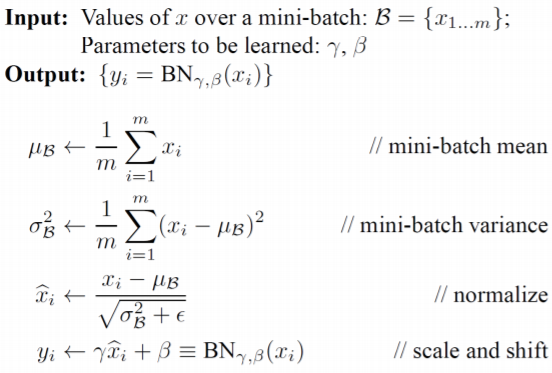
\includegraphics[width=.5\textwidth]{09/17_27}
    \caption{Statistics calculation on mini-batches.}	
\end{figure}
The batchnorm transformation makes each training example \emph{interact} with the \emph{other examples} in each mini-batch,
transforming each data point wrt to the other data points in the mini-batch.

\paragraph{Properties}
Typically, batchnorm is applied right before the nonlinearity:
\begin{equation}
    \sigma(\mathbf{Wx}+\mathbf{b}) ~~~\textrm{becomes}~~~ \sigma \circ \mathrm{BN}_{\gamma,\beta}(\mathbf{Wx})
\end{equation}  
The \emph{bias} can be removed, since when doing the mean subtraction it undoes 
any shift that has been applied. If the shift was needed to have an optimal solution
to the network, the new shift is the $\color{darkred}\beta_i$.

At \emph{test} time it is not possibile to transform a data point wrt to the \emph{mean} and \emph{variance} of the \emph{mini-batch}, because mini-batches are not legitimate. During training a batchnorm layer estimates the mean and variance of the training set and stores them. Since the statistics of different minibatches will likely be different, some king of moving average is kept. At test time the mean and variance used for the normalization of a data point are these averages of the statistics estimated during training.

Beneficial properties include:
\begin{itemize}
    \item Since in each epoch a sample may end up in different minibatches, each time the sample will be transformed in a slightly different way, depending on the mean and 
    variance of the mini-batch that contains it (so depending on the \emph{interaction} with the \emph{other examples} in the mini-batch). 
    Therefore, the stochastic uncertainty of the batch statistics acts as a \emph{regularizer} that can \emph{benefit generalization}: the network tends to become more robust to variations.
    
    \item Batchnorm leads to more \emph{stable gradients}, meaning that one can increase the learning rate and thus achieve \emph{faster training} with more safety.
\end{itemize}

\paragraph{Variants}
Some tried to bring variations to the normalization idea, since it has been argued that normalizing along the \emph{batch dimension} can lead to inconsistency:
\begin{itemize}
    \item Bad transfer across different data distributions. If the training has been made on a certain data distribution, then the network won't transfer well on completely new data. 
    \item The stats must be reliable. The size of the mini-batch determines the quality of the mean and variance estimates; reducing the \emph{mini-batch size} increases the model error dramatically.
\end{itemize}

For this reasons, several variants have been proposed:

\begin{figure}[H]
    \centering
    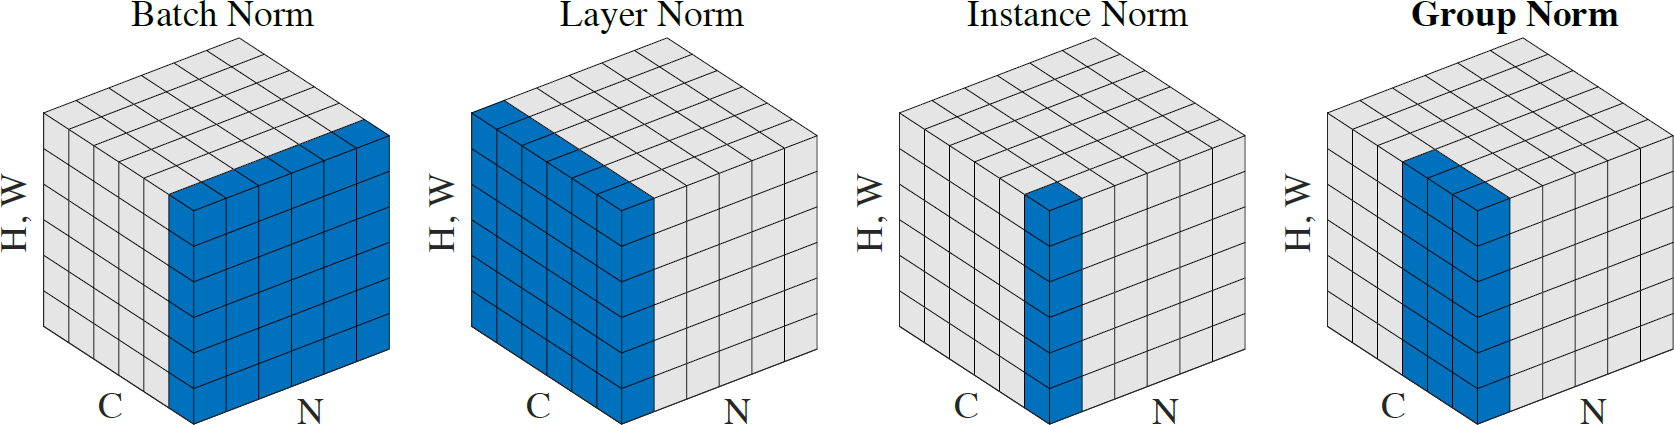
\includegraphics[width=.8\textwidth]{09/nors}
    \caption{Visualization of the action of batchnorm and its variants on the incoming batches of matrices.}
    \label{fig:09:3:batchnorm-visualization}
\end{figure}

Looking at \cref{fig:09:3:batchnorm-visualization}, suppose we have a minibatch of $N$ samples, with each sample being a tensor of dimensions $(H, W, C)$ (e.g. an RGB image, with the spatial dimensions $H, W$ flattened). Then:
\begin{itemize}
    \item \textbf{Batchnorm}: Normalizing each channel independently along the direction of the batch.
    \item \textbf{Layer norm}: Normalizing each sample independently along the direction of the channels.
    \item \textbf{Instance norm}: Normalizing each channel of each sample independently.
    \item \textbf{Group norm}: Normalizing across the channels of each sample, but within some radius.
\end{itemize}